\begin{center}
\fbox{\fbox{\parbox{6.5in}{\centering
\begin{flushleft}

\vspace{2mm}
\hspace{5mm}
\textbf{\underline{Hulknurkade sarnasus}}

\vspace{2mm}
\hspace{5mm}
Kaks kujundit on sarnased, kui nende vastavad nurgad on võrdsed ning vastavad lõigud võrdelised.

\vspace{2mm}
\hspace{5mm}
\begin{tikzpicture}[scale=0.8]

\coordinate (A) at (0,0);
\coordinate (B) at (5,0);
\coordinate (C) at (2,3);

\path (A)--(B) coordinate[pos=0.5](c);
\path (B)--(C) coordinate[pos=0.5](a);
\path (C)--(A) coordinate[pos=0.5](b);

\draw (A)--(B)--(C)--cycle;
\node[below] at (c){$c$};
\node[above right] at (a){$a$};
\node[above left] at (b){$b$};

\node[below] at (A){$A$};
\node[below] at (B){$B$};
\node[above] at (C){$C$};

\pic [draw,angle radius=8mm] {angle=B--A--C} node at(0.45,0.25) {$\alpha$};
\pic [draw,angle radius=7mm] {angle=A--C--B} node at(2,2.5) {$\gamma$};
\pic [draw,angle radius=8mm] {angle=C--B--A} node at(4.3,0.25) {$\beta$}; 

\end{tikzpicture}
\hspace{25mm}
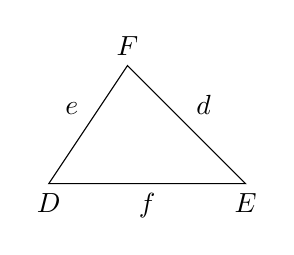
\begin{tikzpicture}[scale=0.5]

\coordinate (A) at (0,0);
\coordinate (B) at (5,0);
\coordinate (C) at (2,3);

\path (A)--(B) coordinate[pos=0.5](c);
\path (B)--(C) coordinate[pos=0.5](a);
\path (C)--(A) coordinate[pos=0.5](b);

\draw (A)--(B)--(C)--cycle;
\node[below] at (c){$f$};
\node[above right] at (a){$d$};
\node[above left] at (b){$e$};

\node[below] at (A){$D$};
\node[below] at (B){$E$};
\node[above] at (C){$F$};


\end{tikzpicture}





\vspace{2mm}
\hspace{5mm}
Järelikult kaks kolmnurka on sarnased, kui:

\begin{itemize}
\item $\angle A = \angle D = \alpha$, $\angle B= \angle E= \beta$, $\angle C = \angle F= \gamma$
\item $\dfrac{d}{a}=\dfrac{e}{b}=\dfrac{f}{c}=k$, kus $k$ on sarnasustegur.
\end{itemize}


\vspace{2mm}
\hspace{5mm}
\textbf{\underline{Kolmnurga sarnasuse tunnused}}

\vspace{5mm}
\hspace{5mm}
\textbf{KKK (külg-külg-külg)}

\vspace{2mm}
\hspace{5mm}
Kaks kolmnurka on sarnased, kui ühe kolmnurga kolm külge on võrdelised teise kolmnurga vastavate\\ \hspace{5mm} külgedega.

\vspace{2mm}
\hspace{5mm}
\textbf{KNK (külg-nurk-külg)}

\vspace{2mm}
\hspace{5mm}
Kaks kolmnurka on sarnased, kui ühe kolmnurga kaks külge on võrdelised teise kolmnurga kahe küljega\\ \hspace{5mm} ja nende külgede vahelised nurgad on võrdsed.

\vspace{2mm}
\hspace{5mm}
\textbf{NN (nurk-nurk)}

\vspace{2mm}
\hspace{5mm}
Kaks kolmnurka on sarnased, kui ühe kolmnurga kaks nurka on vastavalt võrdsed teise kolmnurga kahe\\ \hspace{5mm} nurgaga.


\vspace{5mm}
\hspace{5mm}
\textbf{\underline{Sarnaste hulknurkade ümbermõõt}}

\vspace{2mm}
\hspace{5mm}
Sarnaste hulknurkade ümbermõõtude suhe on võrdne sarnasusteguriga $k$.

\vspace{2mm}
\hspace{5mm}
Ehk:
\begin{equation}
\boxed{\dfrac{P_{2}}{P_{1}}=k}
\end{equation}

\vspace{2mm}
\hspace{5mm}
kus $k$ on sarnasustegur, $P_{1}$ on esimese sarnase hulknurga ümbermõõt ning $P_{2}$ on teise sarnase\\ \hspace{5mm} hulknurga ümbermõõt.


\end{flushleft}
}}}
\end{center}


\pagebreak
\begin{center}
\fbox{\fbox{\parbox{6.5in}{\centering
\begin{flushleft}

\vspace{5mm}
\hspace{5mm}
\textbf{\underline{Sarnaste hulknurkade pindala}}

\vspace{2mm}
\hspace{5mm}
Sarnaste hulknurkade pindalade suhe on võrdne sarnasusteguriga $k^{2}$.

\vspace{2mm}
\hspace{5mm}
Ehk:
\begin{equation}
\boxed{\dfrac{S_{2}}{S_{1}}=k^{2}}
\end{equation}

\vspace{2mm}
\hspace{5mm}
kus $k^{2}$ on sarnasustegur ruudus, $P_{1}$ on esimese sarnase hulknurga pindala ning $P_{2}$ on teise sarnase\\ \hspace{5mm} hulknurga pindala.


\vspace{5mm}
\hspace{5mm}
\textbf{\underline{Mõõtkava}}

\vspace{2mm}
\hspace{5mm}
Mõõtkava näitab, mitu korda on mudeli (nt kaardi) suurused vähendatud või suurendatud võrreldes\\ \hspace{5mm} tõeliste suurustega.

\vspace{2mm}
\hspace{5mm}
\textbf{Arvmõõt} - esitatakse suhtena $1:n$, kus $n$ näitab mitu korda on tegelikke vahemaid plaanil\\ \hspace{5mm} vähendatud.

\vspace{2mm}
\hspace{5mm}
Näiteks: $1:500$ näitab, et $1$ cm plaanil vastab looduses $200$ cm $=$ $2$ m.\\ \hspace{5mm} $1:10 000$ näitab, et $1$ cm plaanil vastab looduses $10 000$ cm $=$ $100$ m .

\vspace{2mm}
\hspace{5mm}
\textbf{Joonmõõt} - Kaardil kujutatakse mõni lõik ning sellele lõigule vastav tegelik pikkus.

\vspace{2mm}
\hspace{5mm}
Näiteks: 

\vspace{5mm}
\hspace{5mm}
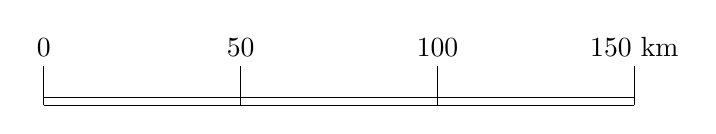
\begin{tikzpicture}[scale=0.5]
\draw (0,0) to (15,0);
\draw (0,0.2) to (15,0.2);
\draw (0,0) to (0,1);
\draw (5,0) to (5,1);
\draw (10,0) to (10,1);
\draw (15,0) to (15,1);

\node[above] at (0,1){$0$};
\node[above] at (5,1){$50$};
\node[above] at (10,1){$100$};
\node[above] at (15,1){$150$ km};
\end{tikzpicture}

\vspace{2mm}
\hspace{5mm}
Kahe jaotise vahel olevale lõigule vastab $50$ km. 
Eeldusel, et jaotiste vaheline lõik on pikkusega 2.5 cm, \\ \hspace{5mm} siis võib leida ka sellele vastav arvmõõt. 

\vspace{2mm}
\hspace{5mm}
$2.5$ cm : 5 000 000 cm =$ \left[\begin{tabular}{c}
Jagame mõlemad\\
pooled 2.5 - ga
\end{tabular} \right] $ =$1$ cm : 2 000 000 cm = 1 : 2 000 000.


\end{flushleft}
}}}
\end{center}
\vspace{0.5cm}

\textbf{Märkmed}\\
\vspace{2mm}
\begin{mdframed}[style=graphpaper]
\vspace{6cm}
\end{mdframed}